\documentclass[12pt, man, a4paper, floatsintext]{apa7}
    
\usepackage[utf8]{inputenc}
\usepackage{csquotes}
\usepackage{amsmath, amssymb}

\usepackage{graphicx}
\graphicspath{{../figures/}}

\usepackage[style=apa, sortcites=true, backend=biber]{biblatex}
\addbibresource{references.bib}


\title{A Machine Learning Approach to Equity Bubble Detection and Market Crash Prediction}
\shorttitle{Machine Learning to Bubble Detection}
\author{Hongkai Yu}
\affiliation{Vancouver School of Economics, University of British Columbia
          \\ ECON 490
          \\ Dr. Jonathan Graves
          \\ April 23, 2021}

\abstract{
    This is the abstract section.
}

\begin{document}

    \linespread{1} % for tables

    \maketitle

    \section{Introduction}

Bubbles and financial crashes are important themes of financial markets. Asset bubbles describe the situation where asset prices significantly deviate from their fundamental values. Notable historical bubble includes the Dutch tulip mania in 1637, the dot-com bubble in 1990s, and the US housing bubble in 2000s. Investors who are unaware of the potential risks of bubbles paid huge prices when markets crashed. 

According to people, this happened \parencite{Chat2018}.

    \section{Background}

    \section{Model}

    \subsection{Model selection}

    \subsubsection{Random Forests}


    \paragraph{GDP}

According to people, this happened again \parencite{Chat2018}.

According to people, this happened again \parencite{Chat2018}.

As shown in Figure~\ref{fig:cv}

\begin{figure}
    \centering
    \caption{CV-tuned decision threshold}
    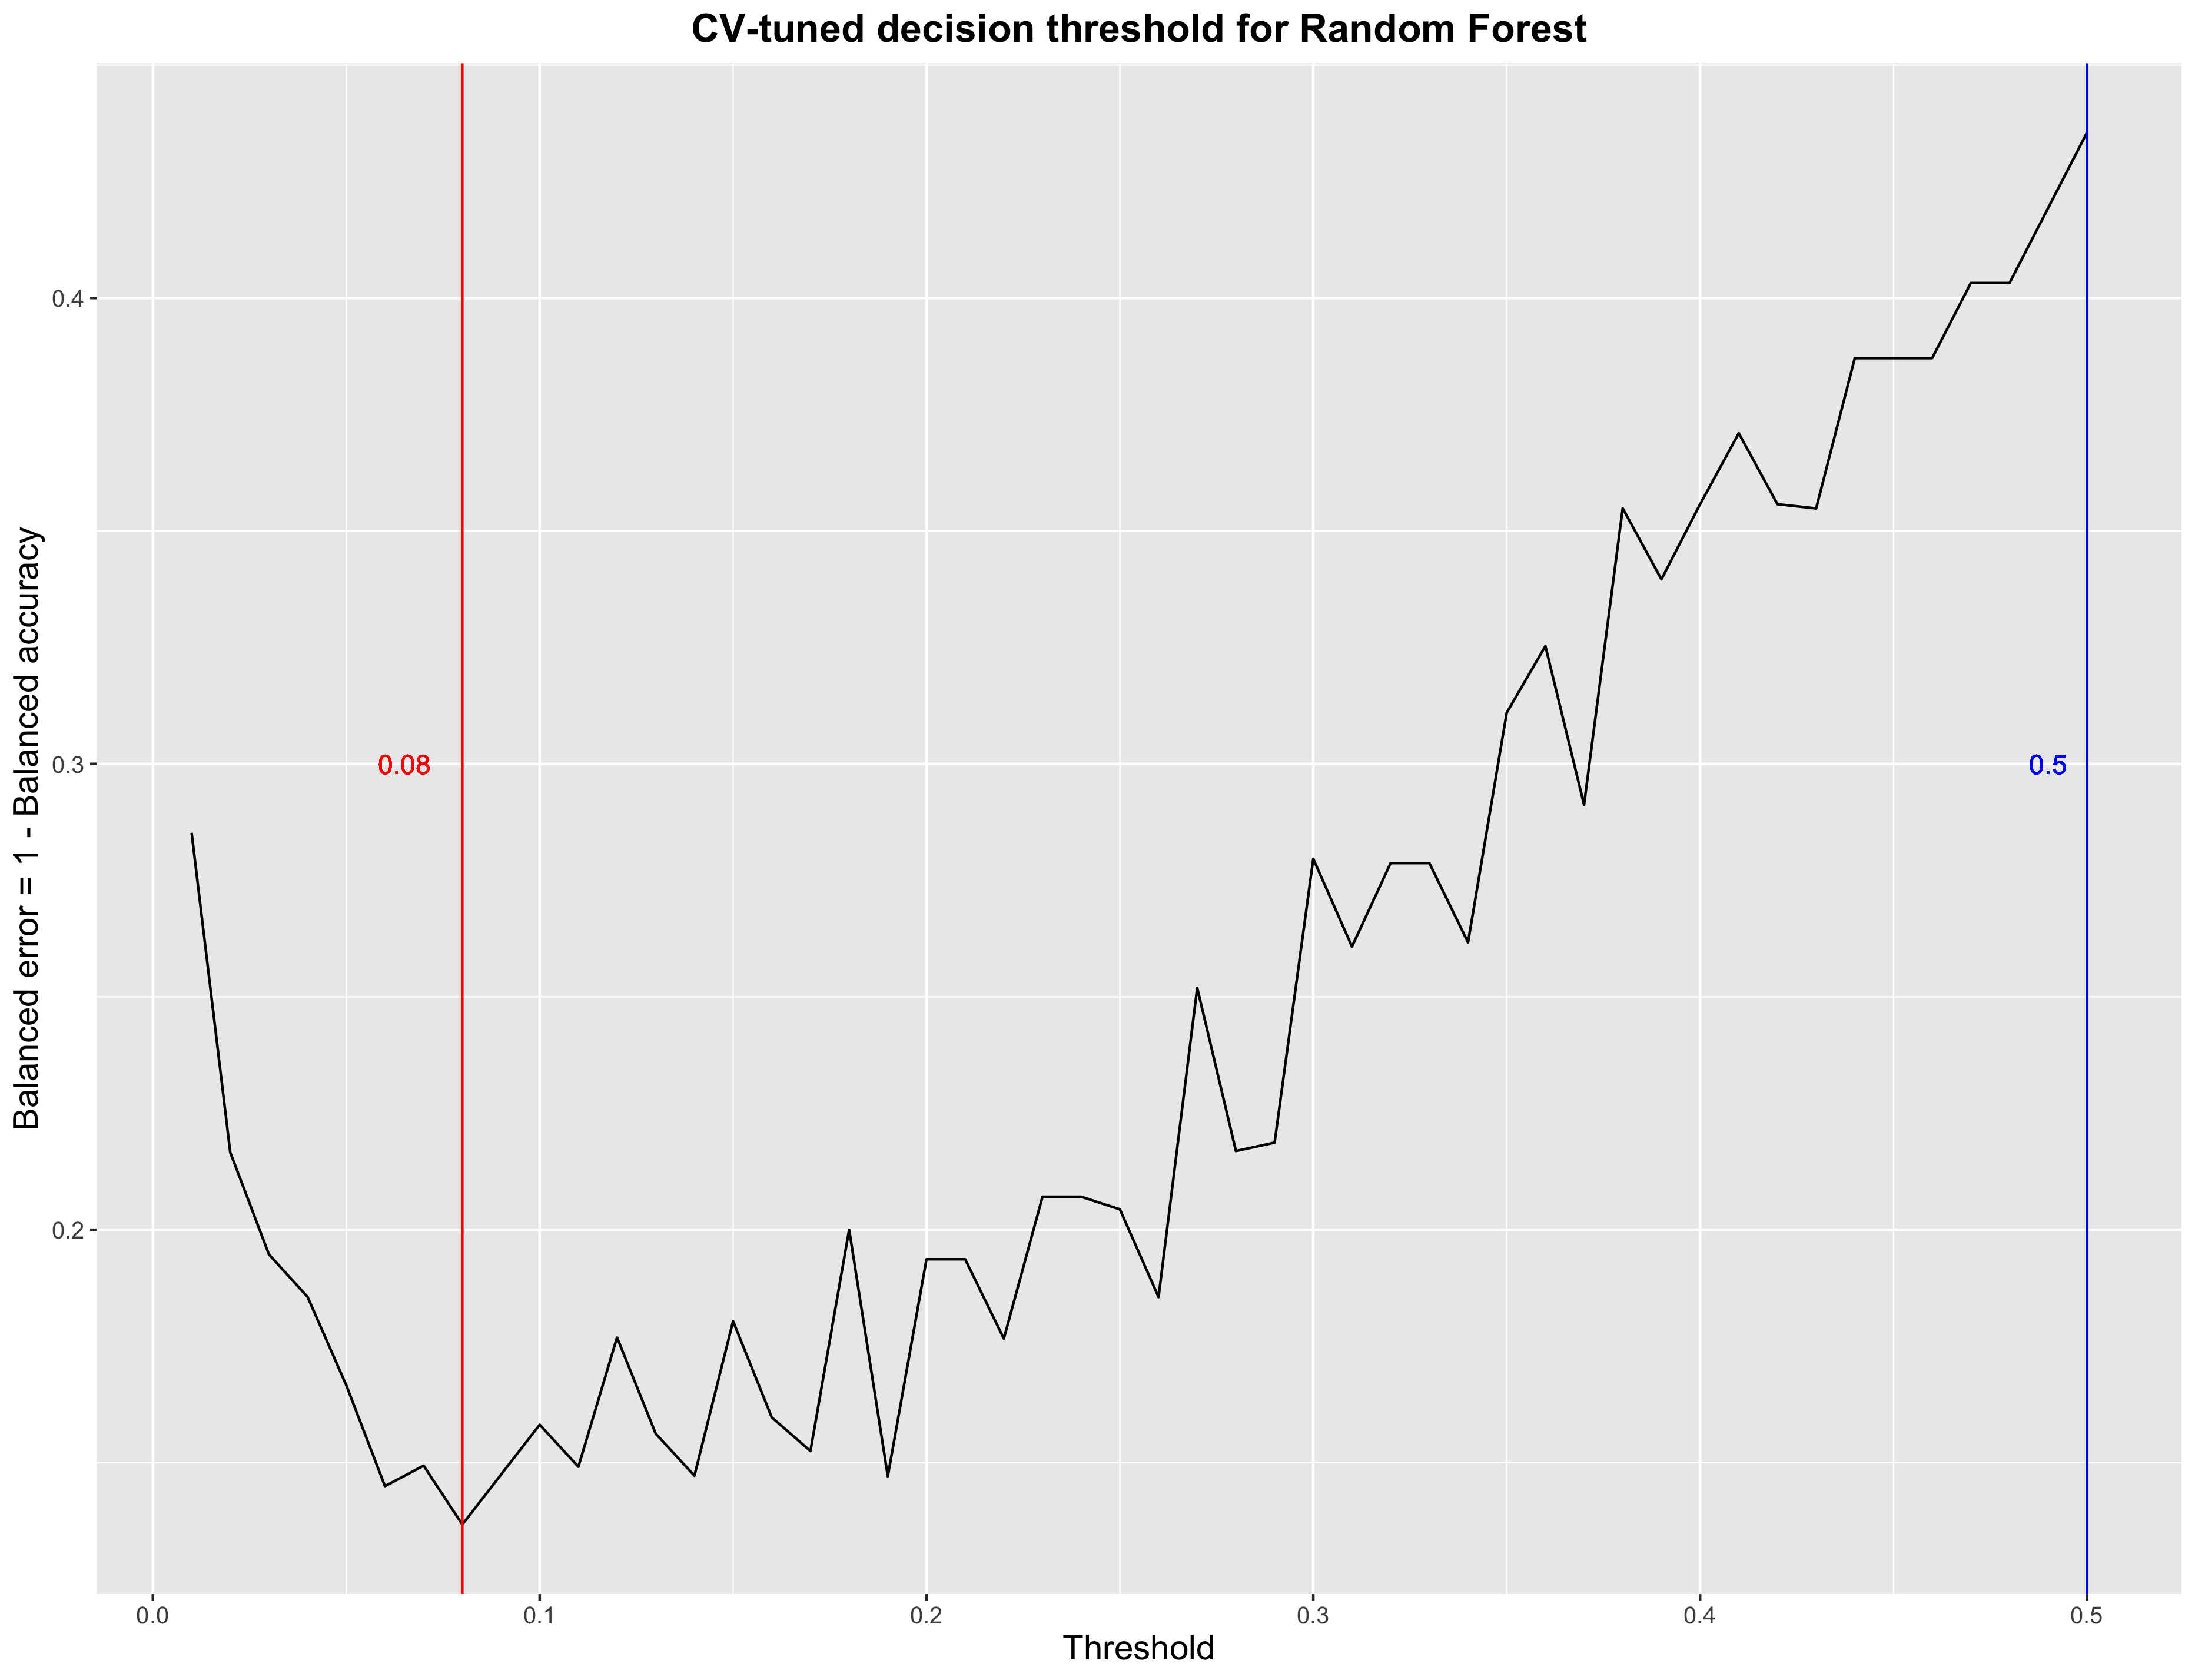
\includegraphics[width=12cm]{cv_threshold}
    \label{fig:cv}
\end{figure}

\begin{figure}
    \centering
    \caption{Variable Importance}
    \includegraphics[width=12cm]{varImpRF}
    \label{fig:varImp}
\end{figure}

According to people, this happened again \parencite{Chat2018}.
As shown in Equation~\ref{eq:logit}

\begin{equation}
    \text{logit}(P(Y)) = \log{\frac{P(Y)}{1-P(Y)}} = X \beta
    \label{eq:logit}
\end{equation}



As shown in Table~\ref{tab:logit}

% Table created by stargazer v.5.2.2 by Marek Hlavac, Harvard University. E-mail: hlavac at fas.harvard.edu
% Date and time: Sat, Apr 17, 2021 - 00:23:32
\begin{table}[!htbp] \centering 
  \caption{} 
  \label{} 
\begin{tabular}{@{\extracolsep{5pt}}lc} 
\\[-1.8ex]\hline 
\hline \\[-1.8ex] 
 & \multicolumn{1}{c}{\textit{Dependent variable:}} \\ 
\cline{2-2} 
\\[-1.8ex] & bubble \\ 
\hline \\[-1.8ex] 
 real\_gdp\_growth & $-$0.007 \\ 
  & (0.035) \\ 
  & \\ 
 inflation & 0.099$^{***}$ \\ 
  & (0.028) \\ 
  & \\ 
 tbill\_yield & 0.237$^{***}$ \\ 
  & (0.073) \\ 
  & \\ 
 shiller\_pe & $-$0.658$^{***}$ \\ 
  & (0.058) \\ 
  & \\ 
 consumer\_confidence & $-$1.182$^{***}$ \\ 
  & (0.147) \\ 
  & \\ 
 mktcap\_gdp\_ratio & 216.592$^{***}$ \\ 
  & (18.361) \\ 
  & \\ 
 sp500\_return & $-$0.105$^{***}$ \\ 
  & (0.033) \\ 
  & \\ 
 sp500\_re3 & 0.018 \\ 
  & (0.022) \\ 
  & \\ 
 sp500\_re6 & $-$0.021 \\ 
  & (0.020) \\ 
  & \\ 
 sp500\_re12 & $-$0.143$^{***}$ \\ 
  & (0.016) \\ 
  & \\ 
 sp500\_re60 & 0.075$^{***}$ \\ 
  & (0.006) \\ 
  & \\ 
 Constant & 106.314$^{***}$ \\ 
  & (13.641) \\ 
  & \\ 
\hline \\[-1.8ex] 
Observations & 1,112 \\ 
Log Likelihood & $-$410.346 \\ 
Akaike Inf. Crit. & 844.693 \\ 
\hline 
\hline \\[-1.8ex] 
\textit{Note:}  & \multicolumn{1}{r}{$^{*}$p$<$0.1; $^{**}$p$<$0.05; $^{***}$p$<$0.01} \\ 
\end{tabular} 
\end{table} 

% \input{df.tex}

According to people, this happened again \parencite{Chat2018}.
According to people, this happened again \parencite{Chat2018}.
According to people, this happened again \parencite{Chat2018}.

    \clearpage

    \printbibliography

\end{document}